\documentclass{article}


% if you need to pass options to natbib, use, e.g.:
%     \PassOptionsToPackage{numbers, compress}{natbib}
% before loading neurips_2023


% ready for submission
% \usepackage{neurips_2023}


% to compile a preprint version, e.g., for submission to arXiv, add add the
% [preprint] option:
%     \usepackage[preprint]{neurips_2023}


% to compile a camera-ready version, add the [final] option, e.g.:
%     \usepackage[final]{neurips_2023}


% to avoid loading the natbib package, add option nonatbib:
   \usepackage[nonatbib]{neurips_2023}


\usepackage[utf8]{inputenc} % allow utf-8 input
\usepackage[T1]{fontenc}    % use 8-bit T1 fonts
\usepackage{hyperref}       % hyperlinks
\usepackage{url}            % simple URL typesetting
\usepackage{booktabs}       % professional-quality tables
\usepackage{amsfonts}       % blackboard math symbols
\usepackage{nicefrac}       % compact symbols for 1/2, etc.
\usepackage{microtype}      % microtypography
\usepackage{xcolor}         % colors
\usepackage{listings}
\usepackage{graphicx}

\usepackage{amssymb}
\usepackage{framed}
\usepackage{geometry}
\usepackage{subfig}         % Required for minipages.
\usepackage{hyperref}       % Required for hyperlinks.
\usepackage{float}
\usepackage[square,numbers]{natbib}
\bibliographystyle{abbrvnat}


\title{DD2424 Project - Group 12 \\ Text Generation}


% The \author macro works with any number of authors. There are two commands
% used to separate the names and addresses of multiple authors: \And and \AND.
%
% Using \And between authors leaves it to LaTeX to determine where to break the
% lines. Using \AND forces a line break at that point. So, if LaTeX puts 3 of 4
% authors names on the first line, and the last on the second line, try using
% \AND instead of \And before the third author name.


\author{%
  % David S.~Hippocampus\thanks{Use footnote for providing further information
  %   about author (webpage, alternative address)---\emph{not} for acknowledging
  %   funding agencies.} \\
  % Department of Computer Science\\
  % Cranberry-Lemon University\\
  % Pittsburgh, PA 15213 \\
  % \texttt{hippo@cs.cranberry-lemon.edu} \\
  % examples of more authors
  % \And
  Tristan PERROT \\
  % Affiliation \\
  % Address \\
  \texttt{tristanp@kth.se} \\
  \And
  Adiren JOUANNY \\
  % Affiliation \\
  % Address \\
  \texttt{jouanny@kth.se} \\
  \And
  Paul MAUDUIT \\
  % Affiliation \\
  % Address \\
  \texttt{mauduit@kth.se} \\
  \And
  Arthur DEPRET \\
  % Affiliation \\
  % Address \\
  \texttt{depret@kth.se} \\
}


\begin{document}


\maketitle


\begin{abstract}
  % The abstract paragraph should be indented \nicefrac{1}{2}~inch (3~picas) on
  % both the left- and right-hand margins. Use 10~point type, with a vertical
  % spacing (leading) of 11~points.  The word \textbf{Abstract} must be centered,
  % bold, and in point size 12. Two line spaces precede the abstract. The abstract
  % must be limited to one paragraph.
  This project concerns the generation of Lewis Carroll-like sentences using different architectures of neural networks (RNN, LSTM, GRU, Transformers). Additionally, we evaluate the results both quantitatively and qualitatively, employing various methods to improve these results. The methods used involve optimizing the hyper-parameters of the networks as well as modifying the input data (such as data augmentation and embedding techniques).
\end{abstract}

\section{Introduction}

The problem we aim to address is natural language generation, commonly used for text prediction/completion, content summarization, and chat-bots. A significant challenge in this field is evaluating the generated data, as there are numerous valid outputs and various qualitative and quantitative methods to assess a model and its outputs.

The main objective of this project is to compare different architectures and their effectiveness in generating coherent text. Additionally, we evaluate overall performance metrics, such as inference time and training time. We will optimize the results of the architectures through hyper-parameters tuning and employ data augmentation to achieve better generalization.

\section{Related work}

Research in natural language generation has advanced significantly with various neural network architectures. Recurrent Neural Networks have been foundational but suffer from limitations like vanishing gradients. Long Short-Term Memory networks address these issues with memory cells and gating mechanisms, that makes it able to handle long-term dependencies. More recently, Transformer architectures allowed parallel processing of text, leading to better performance and efficiency in generating coherent and contextually relevant sentences. 

\section{Data}

\subsection{Original Data}

The data used in this project is the entire text of \textbf{Alice's Adventures in Wonderland} by Lewis Carroll, obtained from the Gutenberg Project. This book contains approximately 26500 words. For our experiments, the text was divided into training, validation, and test sets. The validation test is composed of the second to last chapter and the test set is composed of the last chapter. The training set is the rest of the book.

The preprocessing steps were minimal, focusing primarily on splitting the raw corpus into individual characters, as our initial experiments were conducted at the character level. We created a dictionary to map each character to a unique integer, facilitating the conversion of text into a numerical format suitable for model training. This approach allowed us to capture fine-grained details of the text generation process, though it required careful handling of character sequences to maintain coherence in the generated text.

\subsection{Data augmentation}

As suggested in the guidance, we implemented data augmentation. We used the articles \cite{kaggle} \cite{dataaug} as a guidance to implement it. There are multiple type of data augmentation, such as: random insertion, random deletion, characters replacement, back translation, noise injection. In our situation we choose synonym replacement. This is relatively basic because it consists of replacing randomly some work in a sentence with a synonym. In the appendix A we can see some example of replacement. We choose to augment the text two times, concretely this means that we increase the number of unique words in the vocabulary from 3181 to 5628, that is a 77\%  increase. We could have increase more the number of reformulation but it takes a lot more time for a result that is not better. As we will see after, if we increase the number of reformulation we loose the author's ton. Moreover we need to remember that increasing the number of words, increase the time needed for training.


\section{Libraries used}

We base our work on the \textbf{PyTorch} library to efficiently train our models on GPUs, saving time. For text processing, we used the \textbf{NLTK} library to retrieve and process the data, a crucial step in training models for text generation.

\section{Methods}

\subsection{Training the networks}

Initially, we aimed to begin with the simplest foundation to facilitate comparisons with other architectures. For nearly all the networks, we utilized the Adam optimizer \cite{kingma2017adam} and an embedding layer. The Adam optimizer aids in determining the optimal learning rate throughout the training process, while the embedding layer provides a more effective representation of the inputs in a fixed dimension.
For the training, we also used dropout and layer normalization to get a better training result with more generalization.

\subsection{Generating sequences} 

Several methods are available to generate sequences using Recurrent Neural Networks (RNNs) \cite{schmidt2019recurrent} . We experimented with three of them:

\textbf{Deterministic sampling} involves picking the word with the highest probability at each step. This approach produces the most predictable and coherent text, which is especially useful for tasks requiring high reliability. Additionally, it is straightforward to implement and understand. However, it often results in repetitive and monotonous text, as it tends to overuse common phrases and words, leading to less creative outputs.

\textbf{Temperature sampling} scales the probabilities with a temperature factor before sampling from the new distribution. A temperature value below 1 leads to more predictable generations, while a value above 1 results in less predictable, more diverse, but potentially less grammatically correct outputs. This method allows fine-tuning of the randomness in text generation, enabling a balance between coherence and diversity. Its versatility makes it suitable for different types of content, from highly structured to more creative texts. On the downside, finding the optimal temperature can be challenging and may require extensive experimentation. Additionally, high temperatures can lead to nonsensical or grammatically incorrect sentences.

\textbf{Nucleus sampling} (also known as top-p sampling) defines a threshold \(p\) and only keeps the smallest set of words whose cumulative probability is above this threshold. Words are then sampled from this truncated distribution. This method strikes a balance between determinism and randomness, often resulting in coherent yet diverse text. By eliminating unlikely and potentially irrelevant words, it improves the overall quality of the text. However, it is more complex to implement compared to deterministic sampling, and the choice of threshold \(p\) can significantly impact the output, requiring careful fine-tuning.

Each method has its own advantages and trade-offs, making them suitable for different types of text generation tasks. Deterministic sampling is ideal for scenarios requiring high reliability and consistency, temperature sampling offers flexibility in creativity, and nucleus sampling provides a good balance between the two.


\subsection{Evaluation Metrics}

To evaluate the performance of our text generation models, we used several metrics:

\textbf{Loss:} We primarily monitored cross-entropy loss during training, which measures the difference between the predicted and actual word distributions. Lower loss indicates better model predictions.

\textbf{Type-Token Ratio (TTR):} This metric measures lexical diversity by calculating the ratio of unique words (types) to total words (tokens) in the generated text. A higher TTR indicates more diverse vocabulary.

\textbf{Percentage of Correctly Spelled Words:} This metric evaluates the spelling accuracy of the generated text by comparing each word to a standard dictionary, providing a percentage of correctly spelled words.

\textbf{Perplexity:} Perplexity assesses how well the model predicts a word sequence, with lower values indicating better performance. It is the exponentiated average negative log-likelihood of the predicted word sequence.

\textbf{BLEU Score:} The BLEU score evaluates the quality of generated text by comparing it to reference texts, measuring the precision of matching n-grams. Higher BLEU scores indicate better alignment with human-written text.

Using these metrics, we ensured a comprehensive evaluation of both the training process and the quality of the generated text.


\section{Experiments}

In our experiments, we systematically evaluated various aspects of our text generation models. The primary focus was on comparing different architectures, hyperparameters, and regularization techniques to optimize performance. The experiments were structured as follows:

\subsection{Generation Process}\label{Generation study}

As described earlier, there are several methods to generate texts and we compared them. 

This study was performed on our best model, consisting of a 2-layer LSTM with a 100-dimensional embedding, a context of 200 characters, 512 hidden nodes per layer, a dropout of 0.3 and layer normalization applied between the LSTM and fully connected layer.

Figure \ref{fig:text_generation} shows the different metrics, compared to a reference text.
We see that the deterministic method has the lowest TTR, this is due to the fact that it often falls into a repetition loop. Temperature and nucleus clearly outperforms the deterministic method, and we also see a slight improvement when adding nucleus sampling over the temperature, with perplexity going a bit down, approaching the reference text.   

This is why we use the nucleus sampling method in the following experiment to assess the performance of text generation.

\subsection{Model Architecture Comparison}

We compared the performance of RNN and LSTM networks with one and two layers to evaluate the impact of model complexity and depth on text generation.

LSTM models consistently achieve lower training and validation losses compared to RNNs as can be seen in figure \ref{fig:loss_rnn_lstm}, indicating better learning and generalization. The two-layer LSTM converges faster and reaches a lower loss.

In terms of text metrics, in figure \ref{fig:text_rnn_lstm}, RNNs show higher TTR, suggesting more diverse vocabulary usage. However, LSTMs have higher perplexity, indicating less confident predictions. Despite this, LSTMs generate text with higher spelling accuracy and achieve higher BLEU scores, reflecting closer similarity to the reference text. The two-layer LSTM performs the best overall.

In conclusion, while LSTMs exhibit higher perplexity, they outperform RNNs in terms of loss reduction, text coherence, and accuracy. The two-layer LSTM, in particular, demonstrates superior performance, making it the preferred model for text generation tasks in this comparison. 

\subsection{Hidden Nodes Analysis}

We studied the impact of the number of hidden nodes in the network to balance model complexity and computational efficiency.

Figure \ref{fig:loss_hidden} shows that increasing the number of hidden nodes generally improves validation loss but also increases the risk of overfitting, as indicated by the rise in validation loss after several epochs. To mitigate this, regularization techniques are necessary. Additionally, training larger models is computationally intensive, necessitating careful consideration of resource constraints.

In terms of text metrics, we see in figure \ref{fig:text_hidden} that the TTR score increases with more hidden nodes, indicating more diverse vocabulary usage. Perplexity decreases with more hidden nodes, showing improved model confidence and coherence. Spelling accuracy is highest for the 128-node model, suggesting better vocabulary learning. The BLEU score is relatively high across all models, with smaller models achieving the highest scores.

In conclusion, while increasing hidden nodes can enhance performance, it requires regularization to prevent overfitting and involves higher computational costs. An optimal range of hidden nodes, particularly around 256, appears to balance these factors well.

\subsection{Hyperparameter Tuning}

We explored how batch size affects the learning process. Batch size determines the number of samples processed before updating the model parameters.

As shown in Figure \ref{fig:loss_batch}, increasing the batch size speeds up the training process (in terms of update steps); however, the validation loss tends to increase with larger batch sizes. Training with a lower batch size results in slower training but generally leads to better validation performance.

In terms of text generation metrics, we observe in figure \ref{fig:text_batch}, a batch size of 256 achieved the highest TTR score, indicating more diverse vocabulary usage. Despite having the highest perplexity, this batch size also attained the highest BLEU score, suggesting that it generated text most similar to the reference. The BLEU score and spelling accuracy did not vary significantly with batch size.

In conclusion, while larger batch sizes accelerate training, they may lead to higher validation loss. A batch size of 256 strikes a balance, achieving high diversity and similarity to the reference text.

\subsection{Regularization Technique}

To address overfitting, we experimented with dropout, a regularization technique that randomly sets a fraction of input units to zero at each update during training. This helps prevent the network from becoming too specialized to the training data.

As shown in Figure \ref{fig:loss_dropout}, applying dropout increases the training loss slightly but significantly reduces the validation loss and prevents it from rising too quickly.

In terms of text generation metrics, higher dropout values lead to lower TTR scores according to \ref{fig:text_dropout}, indicating reduced diversity in the generated text. However, dropout improves the percentage of correctly spelled words and slightly increases the BLEU score.

Thus, it is important to find a balance in dropout. For our best model in Experiment 1 (\ref{Generation study}), we selected a dropout value of 0.3 to balance these factors effectively.

\subsection{Number of layers}

We investigated whether increasing network depth improves performance by training 2, 3, and 4 layer networks.

In terms of validation loss (figure \ref{fig:loss_nb_layers}), deeper networks resulted in higher validation losses, indicating increased overfitting with more layers.

However, the text generation metrics present a mixed picture as can be seen in figure \ref{fig:text_nb_layers}. Deeper networks achieved higher BLEU scores and slightly better spelling accuracy, but had lower TTR scores, indicating reduced vocabulary diversity.

While adding regularization techniques might improve the performance of deeper networks, this is beyond the scope of this study.


% \subsection{Regularization Techniques}
% Additionally, layer normalization was implemented to normalize the inputs of each layer, stabilizing the learning process and improving model generalization.

\subsection{Transformer Network}

We developed a transformer-based architecture \cite{vaswani2023attention} comprising an encoder and decoder, utilizing multihead attention mechanisms. The resulting model consists of 2.5 million trainable parameters. In this implementation, we used words as tokens for the input rather than individual characters. This approach proved to be one of our most effective architectures for text generation.

Even though the results are very good for a human, according to our metrics (figure \ref{fig:text_transformer})

\subsection{Data Augmentation}

Finally, we explored data augmentation methods to increase the diversity of our training data. This involved generating additional training samples by applying various transformations to the original data, which aimed to improve the model's robustness and its ability to generalize to unseen data.

We tried to use data augmentation on different model from a simple RNN model, we can understand that it increase the loss from 5.66 to 5.87. But when we analyse the synthesized text qualitatively, a few things have changed:
\begin{itemize}
    \item the model is able to create correct sentences
    \item the model is less repetitive 
    \item the model is less representative of the book
\end{itemize}
We will also next implement it on all our best models. 
We can understand that in every case the loss is higher, as we augment the dataset we are using words that have the same meaning (roughly) but that would not be used by the author so it makes the result more accurate in general but less accurate when we think about writing as the author of the dataset.

To have better results using data augmentation it could be interesting to implement contextualized word embedding \cite{wordrep}.



\section{Results}

The firsts model were really not interesting and we obtain almost random generation (however, some words were understandable even though that was a simple RNN based on char representation) like that:
\begin{lstlisting}[breaklines]
Alice you, yot e, and the n all, S rs. Houcl, int you, ife        of thilled them!ns lillillis
mbis lyou, 'Why en and ang,' and Alich yealligi, th af
mers the med Alichem I tou Hic you armnerie youglaidow yriericemealongNlm every wille, you, and the hrick, you, allown and youadveen ilillembell fong th you, ifutilleem ed solllow!' mear ther shng Mer and QWr ace,' th?lllairie
'it,it,' Ilar ter her wou, inl,' h
mem doingn it thise you, thing I rig
 er ma, as wast ulilled nchilled headved Iled Alring!' A
\end{lstlisting}

With our best LSTM model we obtained: 
\begin{lstlisting}[breaklines]
Alice was a little house, and said 'That's very curious.'
'I won't interrupt at this morning, I suppose?' said Alice.
'It doesn't matter which way you go,' said the Mock Turtle a little three of the jurymen.
'It isn't a fine doesn't matter much,' thought Alice, 'to be a serpents to go by this before, never!'
The Mock Turtle sighed deeply, and the long grass rustled at her arm, and walked off.
'They lived on saying "Come up, and make your face, and the poor little thing!' said the Queen.
'It isn't mad.'
'It's the jury-box,' said Alice.
'Come on!' cried the Gryphon, and the Queen was sitting nearer to say 'What a curious dream!' said the Queen.
'Well, it's a good many little pebbles care, and was sitting on the chimney, and said to the Queen, so that they were getting so sudden change, and the moment Alice was thoroughly puzzled in reply.

\end{lstlisting}

And at the very end, the transformer based model output that:
\begin{lstlisting}[breaklines]
Alice was a good deal worse off than before, as the March Hare had just upset the milk-jug into his plate. Alice did not wish to offend the Dormouse again, so she began very cautiously: 'But I don't understand. Where did they draw the treacle from?' 'You can draw water out of a water-well,' said the Hatter; 'so I should think you could draw treacle out of a treacle-well--eh, stupid?' 'But they were IN the well,' Alice said to the Dormouse, not choosing to notice this last remark. 'Of course they were', said the Dormouse; '--well in.' This answer so confused poor Alice,
\end{lstlisting}

\textbf{TO COMPLETE}

\section{Conclusion}

\textbf{TODO}

\newpage

\bibliography{ref}

\newpage

\section*{Appendix: Experiment 1}
\begin{figure}[H]
    \centering
    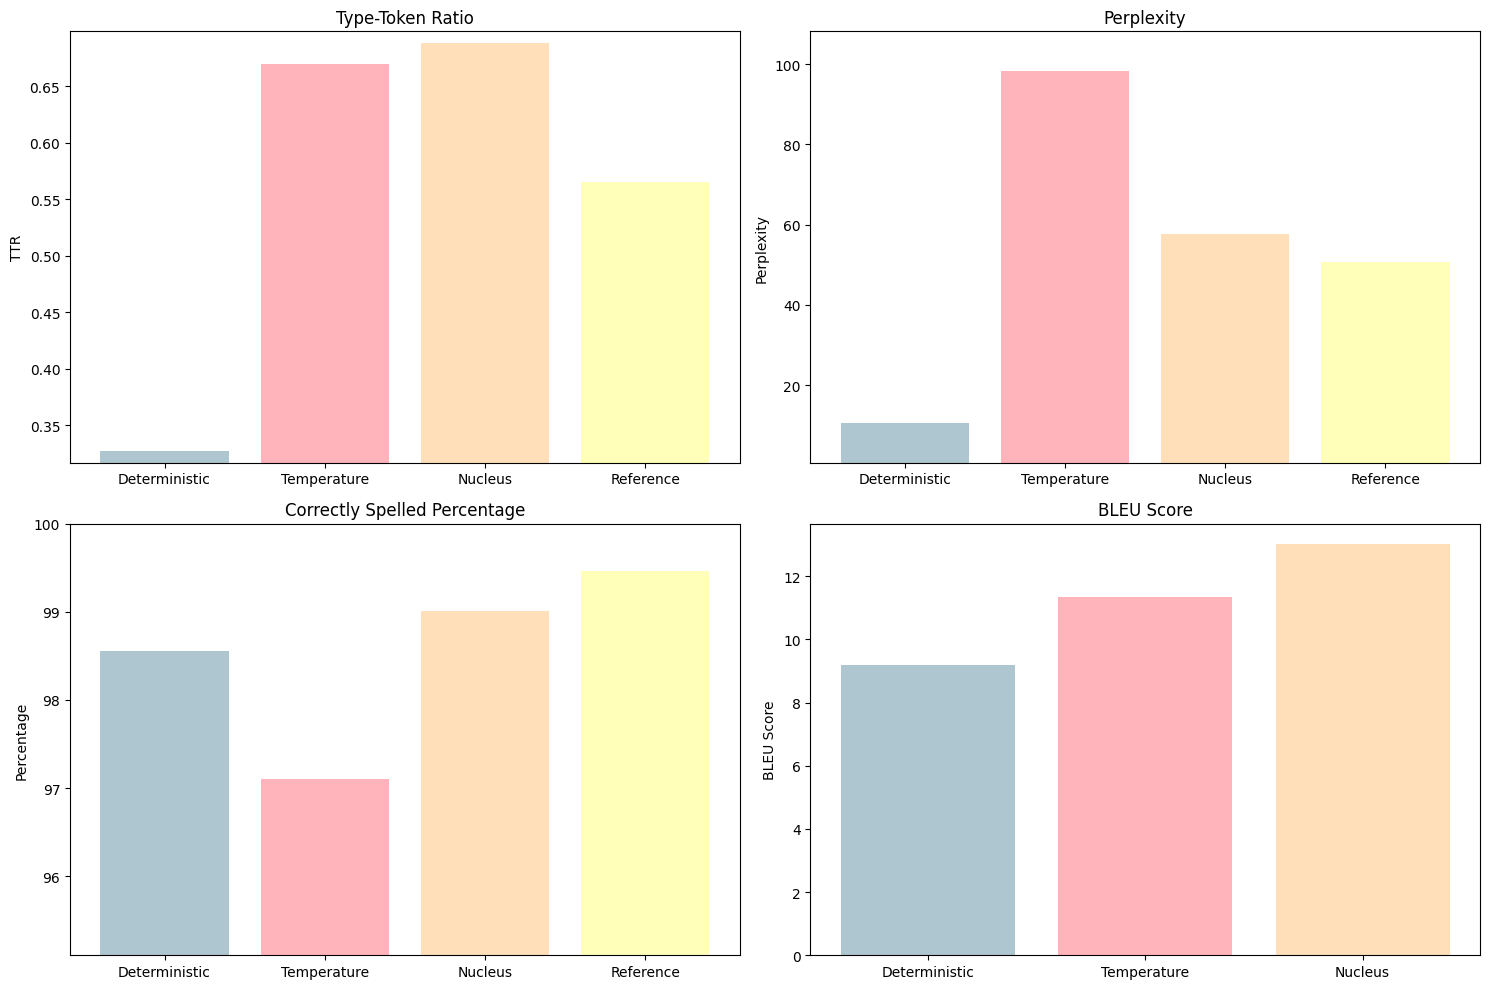
\includegraphics[width=0.8\linewidth]{figures/text_generation.png}
    \caption{Comparison of text generation methods}
    \label{fig:text_generation}
\end{figure}

\section*{Appendix: Experiment 2}
\begin{figure}[H]
    \centering
    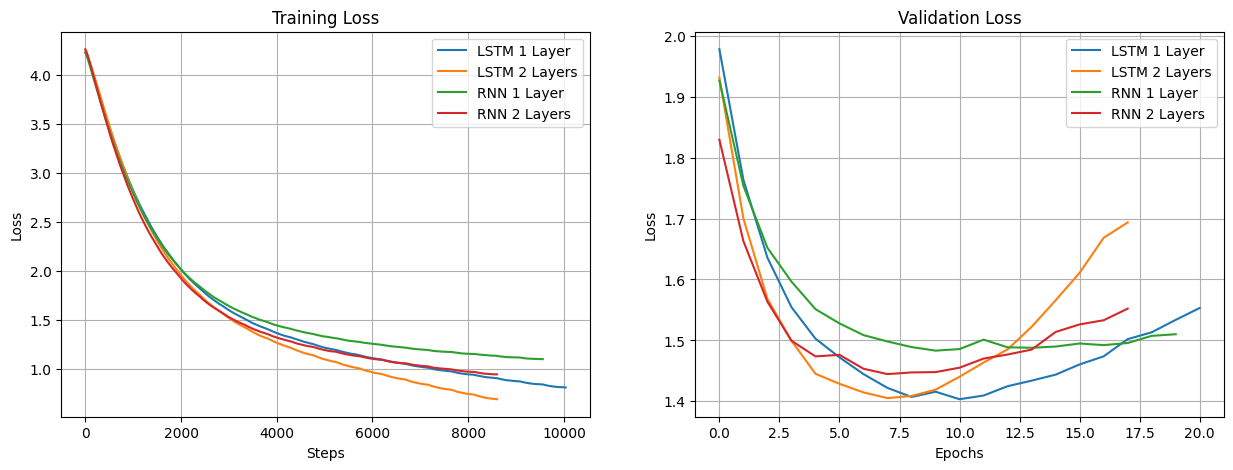
\includegraphics[width=\linewidth]{figures/RNN_LSTM_comparison.png}
    \caption{Losses of RNN and LSTM with 1 or 2 hidden layers}
    \label{fig:loss_rnn_lstm}
\end{figure}

\begin{figure}[H]
    \centering
    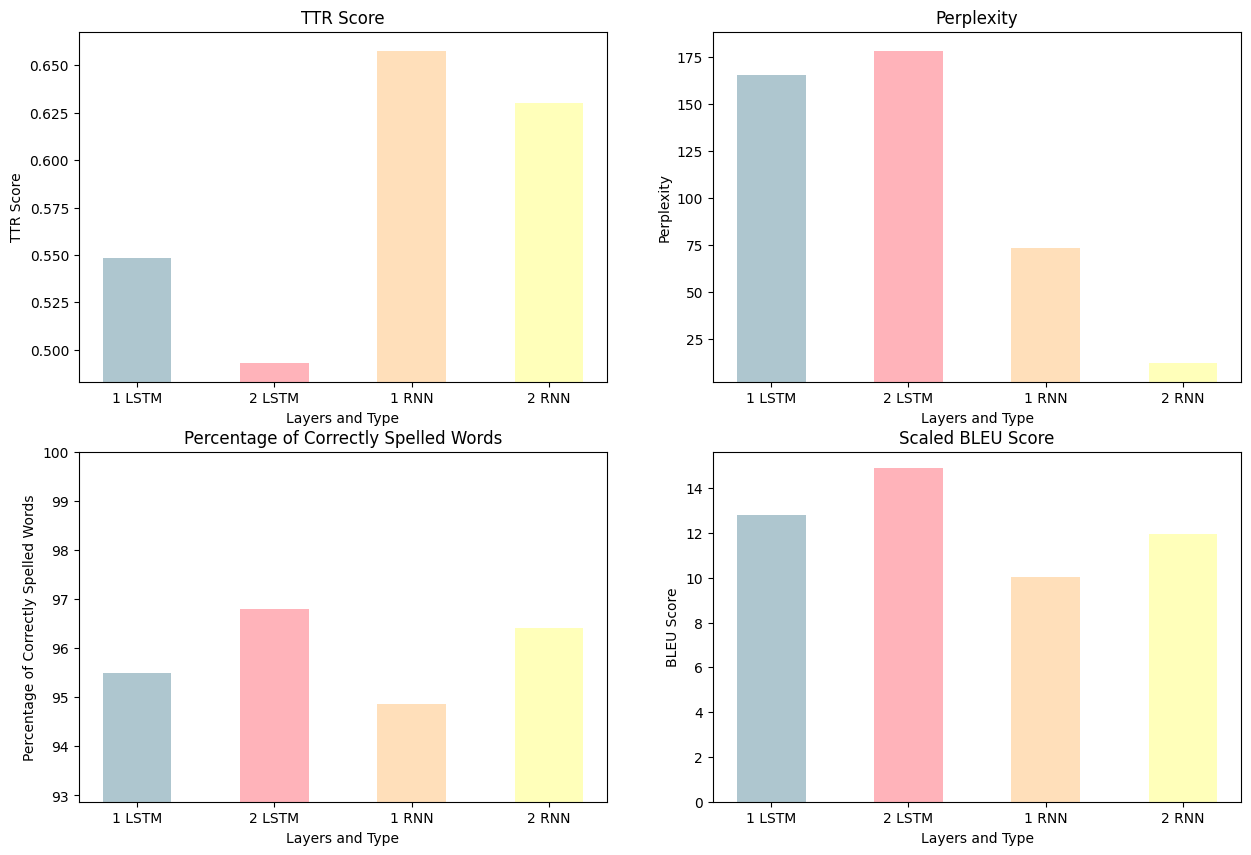
\includegraphics[width=0.8\linewidth]{figures/text_rnn_vs_lstm.png}
    \caption{RNN vs LSTM with 1 or 2 hidden layers}
    \label{fig:text_rnn_lstm}
\end{figure}

\section*{Appendix: Experiment 3}
\begin{figure}[H]
    \centering
    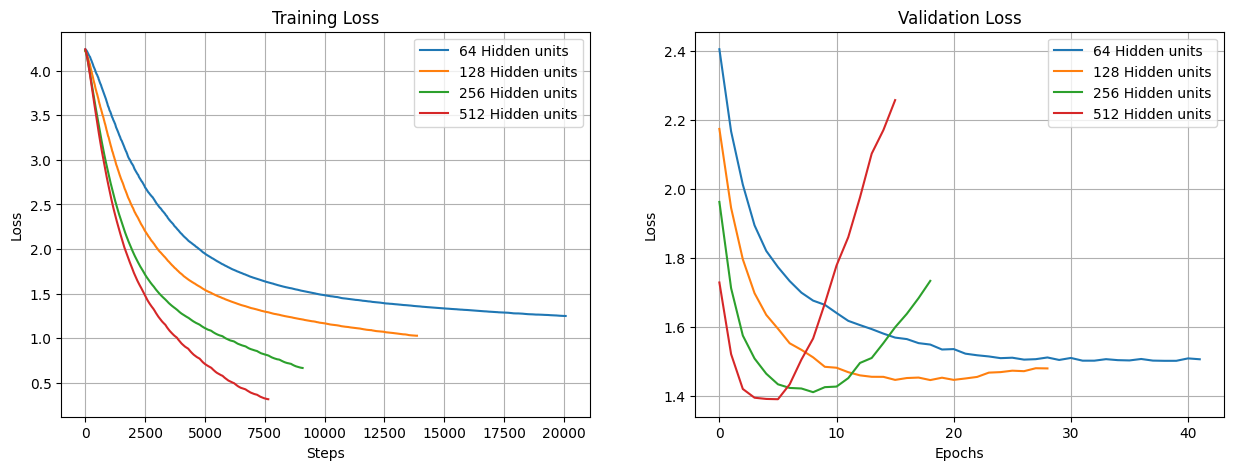
\includegraphics[width=\linewidth]{figures/LSTM_hidden_sizes.png}
    \caption{Losses of LSTM when varying hidden size}
    \label{fig:loss_hidden}
\end{figure}

\begin{figure}[H]
    \centering
    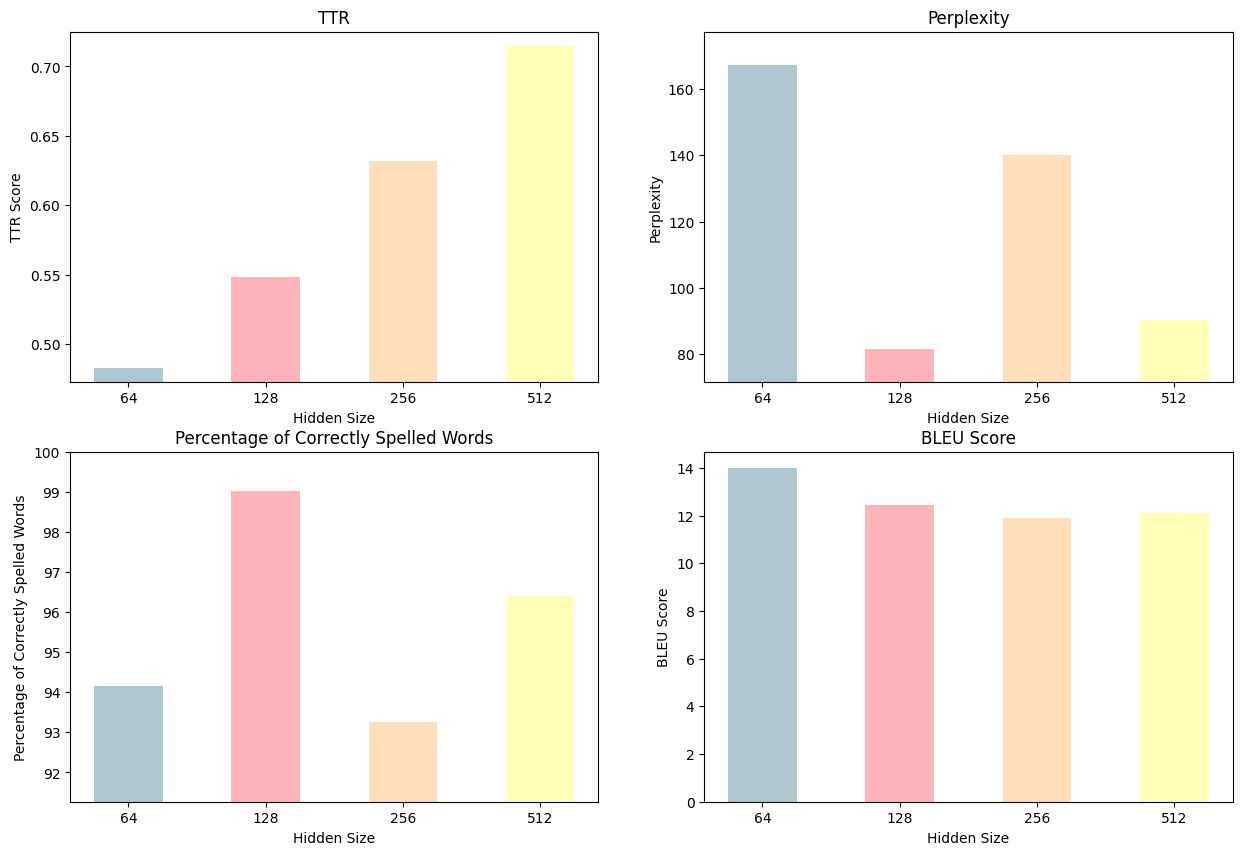
\includegraphics[width=0.8\linewidth]{figures/text_hidden_size.png}
    \caption{Influence of hidden size on text generation}
    \label{fig:text_hidden}
\end{figure}

\section*{Appendix: Experiment 4}
\begin{figure}[H]
    \centering
    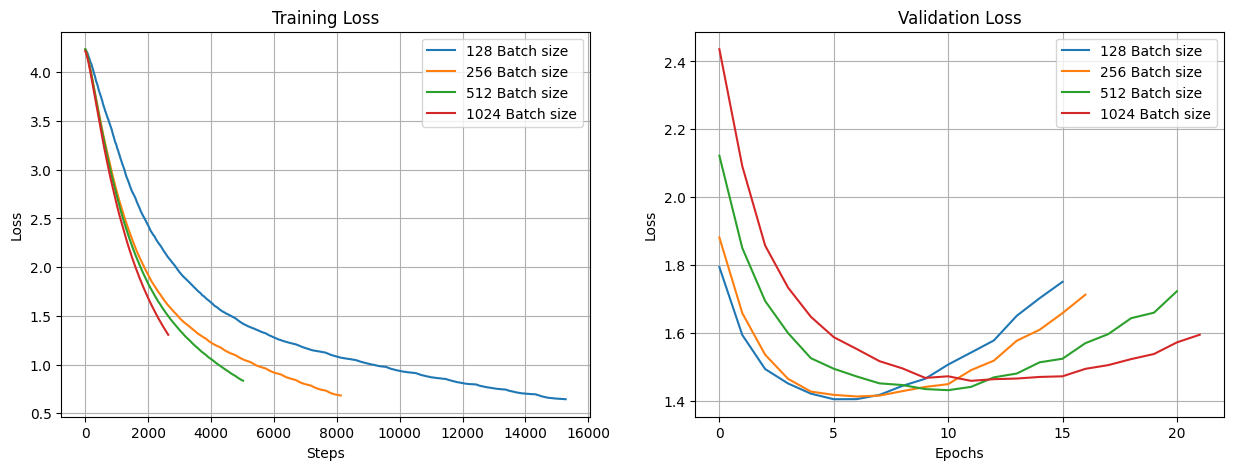
\includegraphics[width=\linewidth]{figures/LSTM_batch_size.png}
    \caption{Losses of LSTM when varying batch size}
    \label{fig:loss_batch}
\end{figure}

\begin{figure}[H]
    \centering
    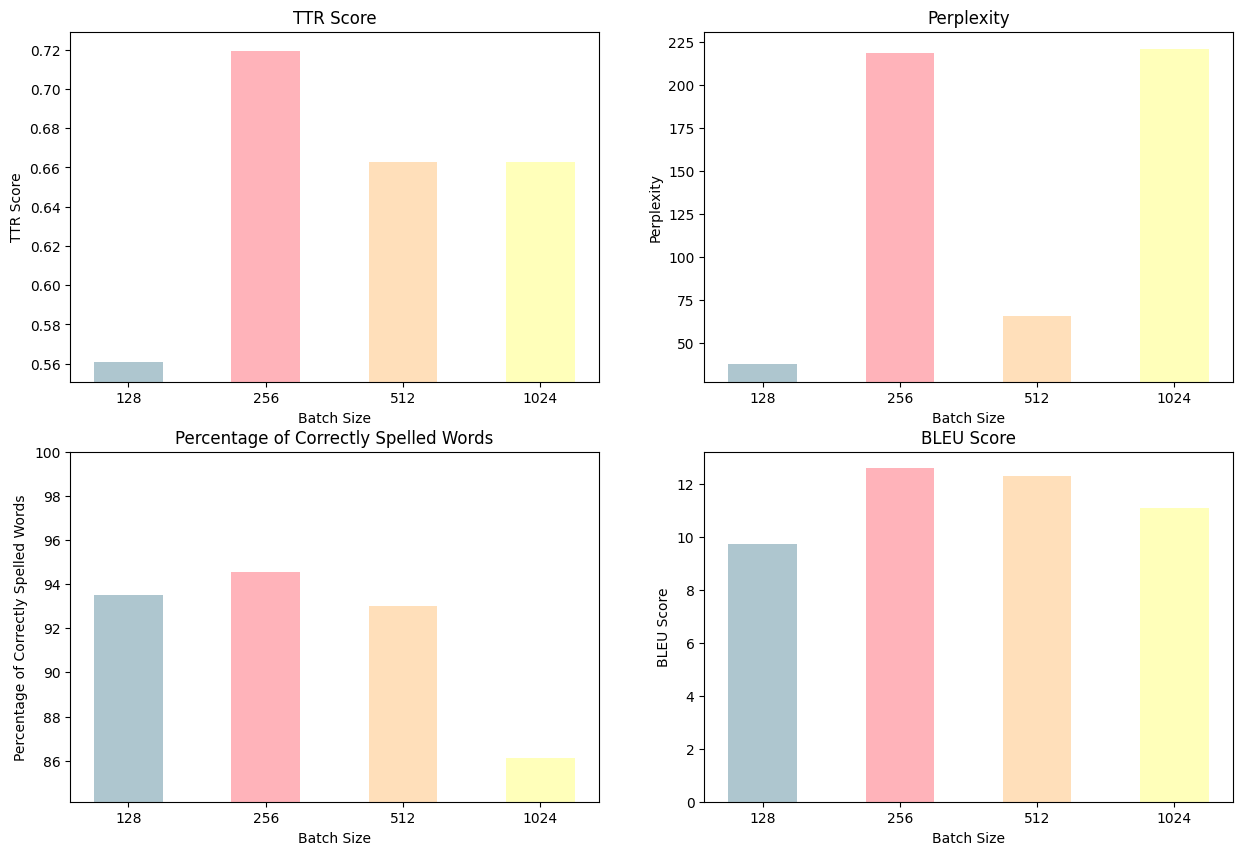
\includegraphics[width=0.8\linewidth]{figures/text_batch_size.png}
    \caption{Influence of batch size on text generation}
    \label{fig:text_batch}
\end{figure}


\section*{Appendix: Experiment 5}
\begin{figure}[H]
    \centering
    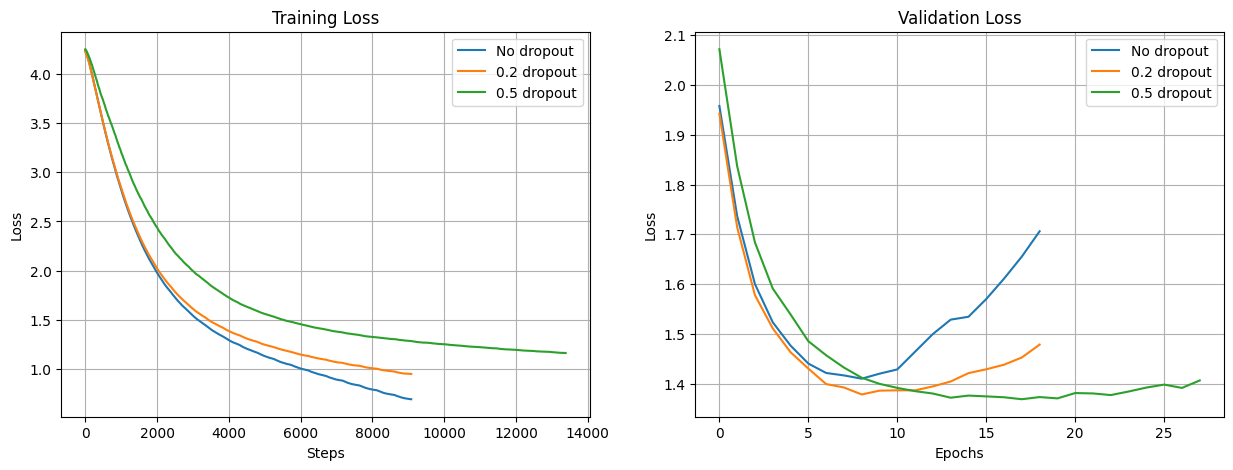
\includegraphics[width=\linewidth]{figures/LSTM_dropout.png}
    \caption{Losses of LSTM when varying the dropout rate}
    \label{fig:loss_dropout}
\end{figure}

\begin{figure}[H]
    \centering
    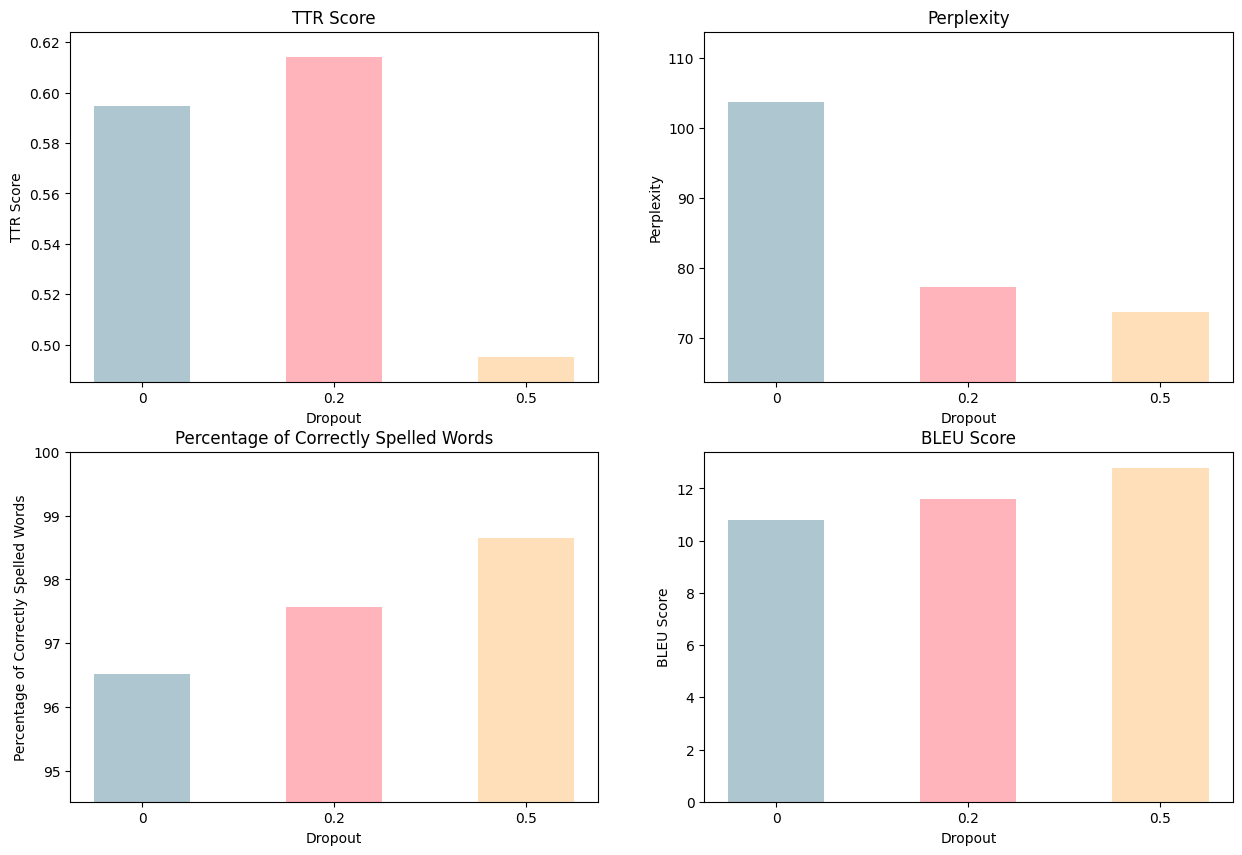
\includegraphics[width=0.8\linewidth]{figures/text_dropout.png}
    \caption{Influence of drop out rate on text generation}
    \label{fig:text_dropout}
\end{figure}

\section*{Appendix: Experiment 6}
\begin{figure}[H]
    \centering
    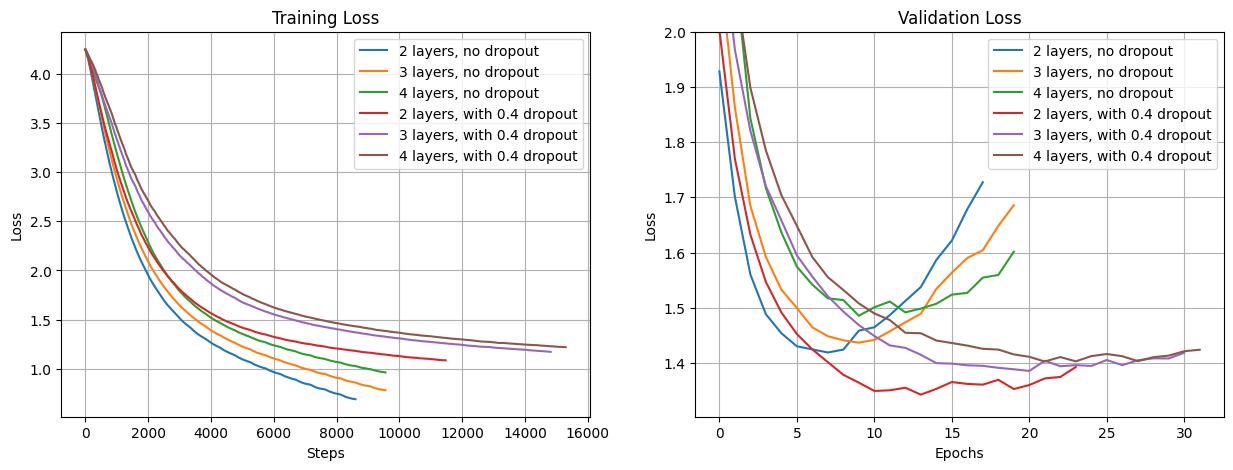
\includegraphics[width=\linewidth]{figures/LSTM_nb_layers.png}
    \caption{Losses of LSTM when varying the number of hidden layers}
    \label{fig:loss_nb_layers}
\end{figure}

\begin{figure}[H]
    \centering
    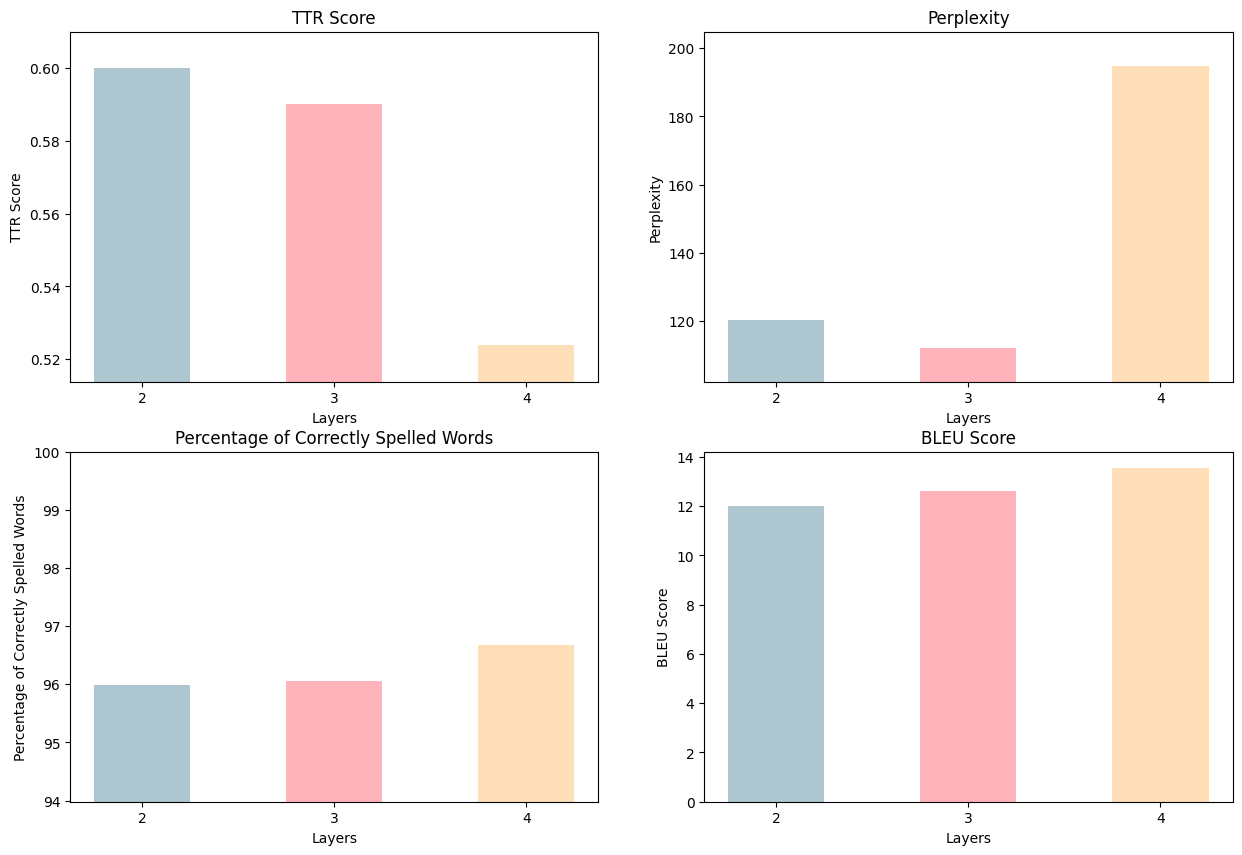
\includegraphics[width=0.8\linewidth]{figures/text_nb_layers.png}
    \caption{Influence of the number of hidden layers on text generation}
    \label{fig:text_nb_layers}
\end{figure}

\section*{Appendix: Experiment 7}

\begin{figure}[H]
    \centering
    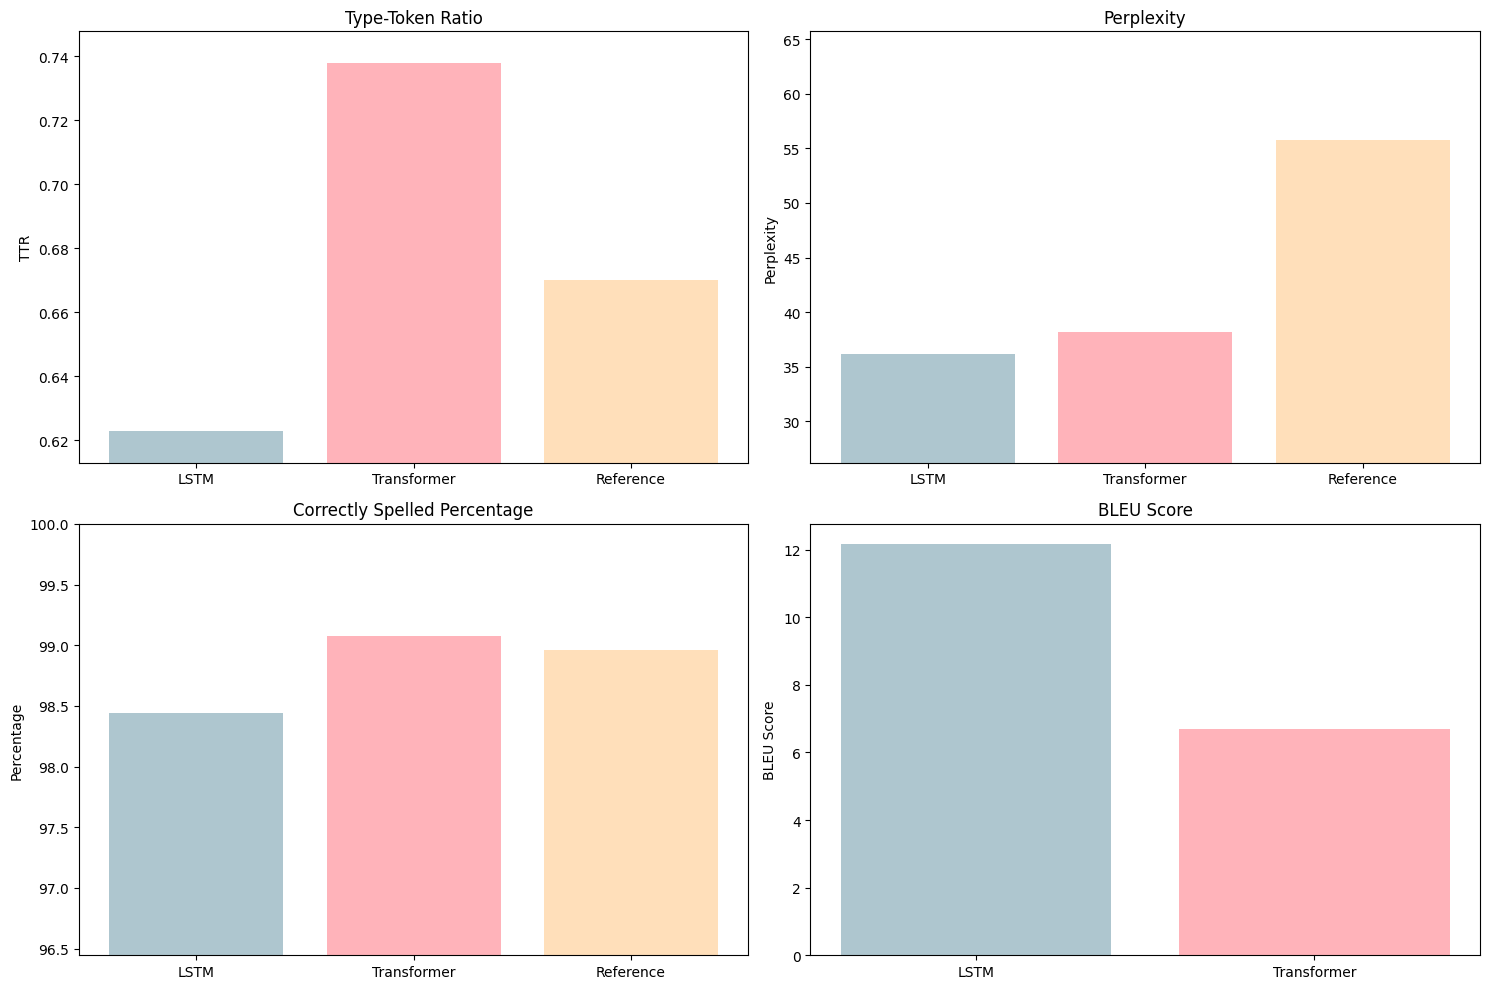
\includegraphics[width=0.8\linewidth]{figures/text_transformers.png}
    \caption{Comparison of text generation: LSTM vs Transformer}
    \label{fig:text_transformer}
\end{figure}

\section*{Appendix: Experiment 8}
% \section{Appendix A: Data augmentation example and graphs}

Here is a short example of the substitution that have been made to augment the dataset.
Example 1 of substitution:
\begin{itemize}
    \item Original: for the hot day made her feel very sleepy and stupid
    \item Reformulated once: for the hot the made her feel not sleepy years stupid
    \item Reformulated twice: for when top day made her feel very sleepy and dumb
\end{itemize}
Example 2 of substitution:
\begin{itemize}
    \item Original: and looked at it 
    \item Reformulated once: and looked at being 
    \item Reformulated twice: more looked at it 
\end{itemize}

And here is what a text generation looks like:
\begin{lstlisting}[breaklines]
    alice was all three sides of the house of her and the three gardeners who was the caterpillar took the cook to the thing before she had never doesnt think to alice some called with cat in the way to the baby with a sigh his took nearer in the distance and the party were off if something came with one paw to the mock turtle in the distance but it made me to fancy what the gryphon said was shouted out that she stood well one of the end of its shoes of mouse in silence was a rabbit was over in more little shriek and stupidly until she could not think of an office of the fire and the first same side of the trees had a sort of all the caterpillar and the rabbit was so she did so she began in the air - - what time it to be tried at the confusion that she set off at the mouse began went on of what dark said the pigeon but she sat down again so in the sea so she went on looking at the baby with one eyes and the things growing and said to herself but alice tried to stay down here which he was so suddenly 

\end{lstlisting}

\newpage


\section{Submission of papers to NeurIPS 2023}

Please read the instructions below carefully and follow them faithfully. \textbf{Important:} This year the checklist will be submitted separately from the main paper in OpenReview, please review it well ahead of the submission deadline: \url{https://neurips.cc/public/guides/PaperChecklist}.


\subsection{Style}


Papers to be submitted to NeurIPS 2023 must be prepared according to the
instructions presented here. Papers may only be up to {\bf nine} pages long,
including figures. Additional pages \emph{containing only acknowledgments and
references} are allowed. Papers that exceed the page limit will not be
reviewed, or in any other way considered for presentation at the conference.


The margins in 2023 are the same as those in previous years.


Authors are required to use the NeurIPS \LaTeX{} style files obtainable at the
NeurIPS website as indicated below. Please make sure you use the current files
and not previous versions. Tweaking the style files may be grounds for
rejection.


\subsection{Retrieval of style files}


The style files for NeurIPS and other conference information are available on
the website at
\begin{center}
  \url{http://www.neurips.cc/}
\end{center}
The file \verb+neurips_2023.pdf+ contains these instructions and illustrates the
various formatting requirements your NeurIPS paper must satisfy.


The only supported style file for NeurIPS 2023 is \verb+neurips_2023.sty+,
rewritten for \LaTeXe{}.  \textbf{Previous style files for \LaTeX{} 2.09,
  Microsoft Word, and RTF are no longer supported!}


The \LaTeX{} style file contains three optional arguments: \verb+final+, which
creates a camera-ready copy, \verb+preprint+, which creates a preprint for
submission to, e.g., arXiv, and \verb+nonatbib+, which will not load the
\verb+natbib+ package for you in case of package clash.


\paragraph{Preprint option}
If you wish to post a preprint of your work online, e.g., on arXiv, using the
NeurIPS style, please use the \verb+preprint+ option. This will create a
nonanonymized version of your work with the text ``Preprint. Work in progress.''
in the footer. This version may be distributed as you see fit, as long as you do not say which conference it was submitted to. Please \textbf{do
  not} use the \verb+final+ option, which should \textbf{only} be used for
papers accepted to NeurIPS. 


At submission time, please omit the \verb+final+ and \verb+preprint+
options. This will anonymize your submission and add line numbers to aid
review. Please do \emph{not} refer to these line numbers in your paper as they
will be removed during generation of camera-ready copies.


The file \verb+neurips_2023.tex+ may be used as a ``shell'' for writing your
paper. All you have to do is replace the author, title, abstract, and text of
the paper with your own.


The formatting instructions contained in these style files are summarized in
Sections \ref{gen_inst}, \ref{headings}, and \ref{others} below.


\section{General formatting instructions}
\label{gen_inst}


The text must be confined within a rectangle 5.5~inches (33~picas) wide and
9~inches (54~picas) long. The left margin is 1.5~inch (9~picas).  Use 10~point
type with a vertical spacing (leading) of 11~points.  Times New Roman is the
preferred typeface throughout, and will be selected for you by default.
Paragraphs are separated by \nicefrac{1}{2}~line space (5.5 points), with no
indentation.


The paper title should be 17~point, initial caps/lower case, bold, centered
between two horizontal rules. The top rule should be 4~points thick and the
bottom rule should be 1~point thick. Allow \nicefrac{1}{4}~inch space above and
below the title to rules. All pages should start at 1~inch (6~picas) from the
top of the page.


For the final version, authors' names are set in boldface, and each name is
centered above the corresponding address. The lead author's name is to be listed
first (left-most), and the co-authors' names (if different address) are set to
follow. If there is only one co-author, list both author and co-author side by
side.


Please pay special attention to the instructions in Section \ref{others}
regarding figures, tables, acknowledgments, and references.


\section{Headings: first level}
\label{headings}


All headings should be lower case (except for first word and proper nouns),
flush left, and bold.


First-level headings should be in 12-point type.


\subsection{Headings: second level}


Second-level headings should be in 10-point type.


\subsubsection{Headings: third level}


Third-level headings should be in 10-point type.


\paragraph{Paragraphs}


There is also a \verb+\paragraph+ command available, which sets the heading in
bold, flush left, and inline with the text, with the heading followed by 1\,em
of space.


\section{Citations, figures, tables, references}
\label{others}


These instructions apply to everyone.


\subsection{Citations within the text}


The \verb+natbib+ package will be loaded for you by default.  Citations may be
author/year or numeric, as long as you maintain internal consistency.  As to the
format of the references themselves, any style is acceptable as long as it is
used consistently.


The documentation for \verb+natbib+ may be found at
\begin{center}
  \url{http://mirrors.ctan.org/macros/latex/contrib/natbib/natnotes.pdf}
\end{center}
Of note is the command \verb+\citet+, which produces citations appropriate for
use in inline text.  For example,
\begin{verbatim}
   \citet{hasselmo} investigated\dots
\end{verbatim}
produces
\begin{quote}
  Hasselmo, et al.\ (1995) investigated\dots
\end{quote}


If you wish to load the \verb+natbib+ package with options, you may add the
following before loading the \verb+neurips_2023+ package:
\begin{verbatim}
   \PassOptionsToPackage{options}{natbib}
\end{verbatim}


If \verb+natbib+ clashes with another package you load, you can add the optional
argument \verb+nonatbib+ when loading the style file:
\begin{verbatim}
   \usepackage[nonatbib]{neurips_2023}
\end{verbatim}


As submission is double blind, refer to your own published work in the third
person. That is, use ``In the previous work of Jones et al.\ [4],'' not ``In our
previous work [4].'' If you cite your other papers that are not widely available
(e.g., a journal paper under review), use anonymous author names in the
citation, e.g., an author of the form ``A.\ Anonymous'' and include a copy of the anonymized paper in the supplementary material.


\subsection{Footnotes}


Footnotes should be used sparingly.  If you do require a footnote, indicate
footnotes with a number\footnote{Sample of the first footnote.} in the
text. Place the footnotes at the bottom of the page on which they appear.
Precede the footnote with a horizontal rule of 2~inches (12~picas).


Note that footnotes are properly typeset \emph{after} punctuation
marks.\footnote{As in this example.}


\subsection{Figures}


\begin{figure}
  \centering
  \fbox{\rule[-.5cm]{0cm}{4cm} \rule[-.5cm]{4cm}{0cm}}
  \caption{Sample figure caption.}
\end{figure}


All artwork must be neat, clean, and legible. Lines should be dark enough for
purposes of reproduction. The figure number and caption always appear after the
figure. Place one line space before the figure caption and one line space after
the figure. The figure caption should be lower case (except for first word and
proper nouns); figures are numbered consecutively.


You may use color figures.  However, it is best for the figure captions and the
paper body to be legible if the paper is printed in either black/white or in
color.


\subsection{Tables}


All tables must be centered, neat, clean and legible.  The table number and
title always appear before the table.  See Table~\ref{sample-table}.


Place one line space before the table title, one line space after the
table title, and one line space after the table. The table title must
be lower case (except for first word and proper nouns); tables are
numbered consecutively.


Note that publication-quality tables \emph{do not contain vertical rules.} We
strongly suggest the use of the \verb+booktabs+ package, which allows for
typesetting high-quality, professional tables:
\begin{center}
  \url{https://www.ctan.org/pkg/booktabs}
\end{center}
This package was used to typeset Table~\ref{sample-table}.


\begin{table}
  \caption{Sample table title}
  \label{sample-table}
  \centering
  \begin{tabular}{lll}
    \toprule
    \multicolumn{2}{c}{Part}                   \\
    \cmidrule(r){1-2}
    Name     & Description     & Size ($\mu$m) \\
    \midrule
    Dendrite & Input terminal  & $\sim$100     \\
    Axon     & Output terminal & $\sim$10      \\
    Soma     & Cell body       & up to $10^6$  \\
    \bottomrule
  \end{tabular}
\end{table}

\subsection{Math}
Note that display math in bare TeX commands will not create correct line numbers for submission. Please use LaTeX (or AMSTeX) commands for unnumbered display math. (You really shouldn't be using \$\$ anyway; see \url{https://tex.stackexchange.com/questions/503/why-is-preferable-to} and \url{https://tex.stackexchange.com/questions/40492/what-are-the-differences-between-align-equation-and-displaymath} for more information.)

\subsection{Final instructions}

Do not change any aspects of the formatting parameters in the style files.  In
particular, do not modify the width or length of the rectangle the text should
fit into, and do not change font sizes (except perhaps in the
\textbf{References} section; see below). Please note that pages should be
numbered.


\section{Preparing PDF files}


Please prepare submission files with paper size ``US Letter,'' and not, for
example, ``A4.''


Fonts were the main cause of problems in the past years. Your PDF file must only
contain Type 1 or Embedded TrueType fonts. Here are a few instructions to
achieve this.


\begin{itemize}


\item You should directly generate PDF files using \verb+pdflatex+.


\item You can check which fonts a PDF files uses.  In Acrobat Reader, select the
  menu Files$>$Document Properties$>$Fonts and select Show All Fonts. You can
  also use the program \verb+pdffonts+ which comes with \verb+xpdf+ and is
  available out-of-the-box on most Linux machines.


\item \verb+xfig+ "patterned" shapes are implemented with bitmap fonts.  Use
  "solid" shapes instead.


\item The \verb+\bbold+ package almost always uses bitmap fonts.  You should use
  the equivalent AMS Fonts:
\begin{verbatim}
   \usepackage{amsfonts}
\end{verbatim}
followed by, e.g., \verb+\mathbb{R}+, \verb+\mathbb{N}+, or \verb+\mathbb{C}+
for $\mathbb{R}$, $\mathbb{N}$ or $\mathbb{C}$.  You can also use the following
workaround for reals, natural and complex:
\begin{verbatim}
   \newcommand{\RR}{I\!\!R} %real numbers
   \newcommand{\Nat}{I\!\!N} %natural numbers
   \newcommand{\CC}{I\!\!\!\!C} %complex numbers
\end{verbatim}
Note that \verb+amsfonts+ is automatically loaded by the \verb+amssymb+ package.


\end{itemize}


If your file contains type 3 fonts or non embedded TrueType fonts, we will ask
you to fix it.


\subsection{Margins in \LaTeX{}}


Most of the margin problems come from figures positioned by hand using
\verb+\special+ or other commands. We suggest using the command
\verb+\includegraphics+ from the \verb+graphicx+ package. Always specify the
figure width as a multiple of the line width as in the example below:
\begin{verbatim}
   \usepackage[pdftex]{graphicx} ...
   \includegraphics[width=0.8\linewidth]{myfile.pdf}
\end{verbatim}
See Section 4.4 in the graphics bundle documentation
(\url{http://mirrors.ctan.org/macros/latex/required/graphics/grfguide.pdf})


A number of width problems arise when \LaTeX{} cannot properly hyphenate a
line. Please give LaTeX hyphenation hints using the \verb+\-+ command when
necessary.


\begin{ack}
Use unnumbered first level headings for the acknowledgments. All acknowledgments
go at the end of the paper before the list of references. Moreover, you are required to declare
funding (financial activities supporting the submitted work) and competing interests (related financial activities outside the submitted work).
More information about this disclosure can be found at: \url{https://neurips.cc/Conferences/2023/PaperInformation/FundingDisclosure}.


Do {\bf not} include this section in the anonymized submission, only in the final paper. You can use the \texttt{ack} environment provided in the style file to autmoatically hide this section in the anonymized submission.
\end{ack}







%%%%%%%%%%%%%%%%%%%%%%%%%%%%%%%%%%%%%%%%%%%%%%%%%%%%%%%%%%%%


\end{document}